\documentclass[11pt]{article}  
\usepackage[margin=.5in]{geometry}
\parindent=0in
\parskip=8pt
\usepackage{fancyhdr,amssymb,amsmath, graphicx, listings,float,subfig,enumerate,epstopdf,color,multirow,setspace,bm,textcomp}
\usepackage[usenames,dvipsnames]{xcolor}
\usepackage{hyperref}
%\usepackage{calc}
%\usepackage{tikz}
%\usepackage{mathtools}
%\usetikzlibrary{matrix}
\usepackage{multirow}
\usepackage{graphicx}
\graphicspath{ {./} }


\pagestyle{fancy}


\begin{document} 

\lhead{Assignment \# 4}
\chead{Daniel Frey}
\rhead{\today}

\begin{center}
\begin{Large}
	CS 4720/5720 Design and Analysis of Algorithms \\
	Homework \#4 \\
	Daniel Frey
\end{Large}
\end{center}

\section*{Answers to homework problems:}

\begin{enumerate}
%1
	\item
		\textbf{\textit{Edit Distance Problem}}

		\begin{enumerate}[(a)]
%1a
			\item
				\textbf{Algorithm:} \\
					\hspace*{.5cm}
					Loop through each character in the first string while looping through each character in the second string. If either of the strings are empty, then set the value to the opposite loop counter to indicate the number of operations up to that point. If the previous characters were the same, then use previously generated result. If previous characters were different, then determine if change, insert, or delete. \\ \\
				\textbf{Pseudocode:} \\
					\hspace*{.5cm}
					EditDistanceDP(string1, string2) \\
						\hspace*{1cm}
						m = size string1, n = size string2 \\
						\hspace*{1cm}
						results[m+1, n+1] \\
						\hspace*{1cm}
						for i = 0 to m \\
							\hspace*{1.5cm}
							for j = 0 to n \\
								\hspace*{2cm}
								if i == 0 \\
									\hspace*{2.5cm}
									results[i, j] = j \\
								\hspace*{2cm}
								else if j == 0 \\
									\hspace*{2.5cm}
									results[i, j] = i \\
								\hspace*{2cm}
								else if string1[i-1] == string2[j-1] \\
									\hspace*{2.5cm}
									results[i, j] = results[i-1, j-1] \\
								\hspace*{2cm}
								else \\
									\hspace*{2.5cm}
									results[i, j] = 1 + min(results[i-1, j-1], results[i, j-1], results[i-1, j]) \\
						\hspace*{1cm}
						return results[m, n]
				
%1b
			\item
				\textbf{Time Complexity:} \\		
					\hspace*{.5cm}
					\textbf{Worst-case:} (Two for loops) \\
						\hspace*{1cm}
						$ \sum{_{i=0}^{m} \sum{_{j=0}^{n}}1} = (m+1)(n+1) \in \Theta(mn) $ \\
						
					\hspace*{.5cm}
					\textbf{Best-case} = Worst-case $ \in \Theta(mn) $: must iterate through entirety of each for loop. \\
				
%1c
			\item 
				\textbf{\textit{Code}} \\
				\hspace*{.5cm}
				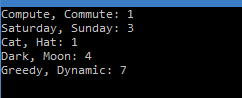
\includegraphics{EditDistanceDP} \\
				
		\end{enumerate}

%2
	\item
		\textbf{\textit{Coin Change Problem}}
	
		\begin{enumerate}[(a)]
%2a		
		\item
			\textbf{\textit{DP Code}} \\
%2b
		\item
			\textit{Greedy Coin Change} \\
			\textit{(Assumption: Denominations D[1...m] in ascending order.)} \\
			
			\begin{enumerate}[(i)]
	%2b.i
				\item
					\textbf{Algorithm: } \\
						\hspace*{.5cm}
						Loop through each coin denomination from largest to smallest. Figure out how many of current largest coin can be used for current value \emph{n}, and subtract that from the current value \emph{n}. \\
					
					\textbf{Pseudocode:} \\
						\hspace*{.5cm}
						CoinChangeGreedy(D[1...m],  n) \\
							\hspace*{1cm}
							numCoins = 0 \\
							\hspace*{1cm}
							 for i = m to 1\\
								\hspace*{1.5cm}
								if n/D[i] $ \geq $ 1 \\
									\hspace*{2cm}
									n = n - [(n/D[i]) * D[i]] \\
									\hspace*{2cm}
									numCoins = numCoins + (n/D[i]) \\
							\hspace*{1cm}
							return numCoins \\

	%2b.ii
				\item
					\textbf{Time complexity:} \\
						\hspace*{.5cm}
						\textbf{Worst-case:} (For loop dependent on m.) \\
							\hspace*{1cm}
							$ \sum_{m}^{1} 1 \in \Theta(m) $ \\
							
						\hspace*{.5cm}
						\textbf{Best-case:} = Worst-case $ \in \Theta(m) $ : must iterate through entirety of for loop. \\
					
	%2b.iii
				\item
					\textbf{\textit{Code}} \\
					
			
			\end{enumerate}
%2c
		\item
			\textbf{Comparison:} \\
			\begin{enumerate}[(i)]
	%2c.i
				\item
					\textbf{Non-optimal Greedy Denominations:} \\
						\hspace*{.5cm}
						\begin{tabular}{ |c|c||c|c| }
							\hline
							\multicolumn{4}{|c|}{\textbf{Minimum Number Coins}} \\
							\hline
							Denomination & $ n $ & DP & Greedy \\
							\hline
							\{1, 5, 6\}& 10 & 2 & 5 \\
							\hline
							\{1, 10, 15\}& 20 & 2 & 6 \\ 
							\hline
							\{1, 30, 50\}& 60 & 2 & 11 \\ 
							\hline
						\end{tabular}
						\vspace{5mm}
					
	%2c.ii
				\item
					\textbf{Sample Comparisons:} \\
		%Denomination {1, 5, 6}
						\hspace*{.5cm}
						\begin{tabular}{ |c||c|c| }
							\hline
							\multicolumn{3}{|c|}{\textbf{Denomination \{1, 5, 6\}}} \\
							\hline
							$ n $ & DP & Greedy \\
							\hline
							250 & 42 & 45 \\
							\hline
							500 & 84 & 85 \\ 
							\hline
							750 & 125 & 125 \\ 
							\hline
							1000 & 167 & 170 \\
							\hline
						\end{tabular}
						\vspace{5mm}
						
		%Denomination {1, 10, 15}
						\hspace*{.5cm}
						\begin{tabular}{ |c||c|c| }
							\hline
							\multicolumn{3}{|c|}{\textbf{Denomination \{1, 10, 15\}}} \\
							\hline
							$ n $ & DP & Greedy \\
							\hline
							250 & 17 & 17 \\
							\hline
							500 & 34 & 38 \\ 
							\hline
							750 & 50 & 50 \\ 
							\hline
							1000 & 67 & 67 \\
							\hline
						\end{tabular}
						\vspace{5mm}

		%Denomination {1, 30, 50}
						\hspace*{.5cm}
						\begin{tabular}{ |c||c|c| }
							\hline
							\multicolumn{3}{|c|}{\textbf{Denomination \{1, 30, 50\}}} \\
							\hline
							$ n $ & DP & Greedy \\
							\hline
							250 & 5 & 5 \\
							\hline
							500 & 10 & 10 \\ 
							\hline
							750 & 15 & 15 \\ 
							\hline
							1000 & 20 & 20 \\
							\hline
						\end{tabular}
						\vspace{5mm}
					
	%2c.iii
				\item
					\textbf{Plot:} \\
					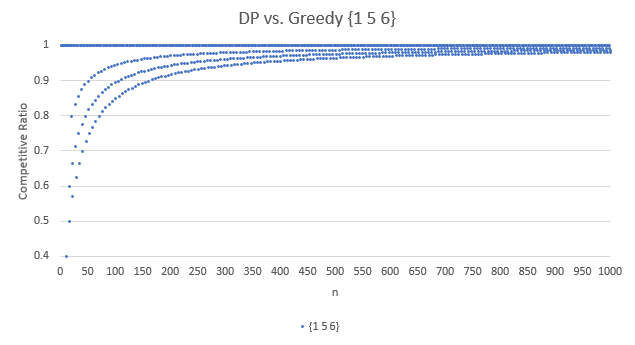
\includegraphics{156} \\
					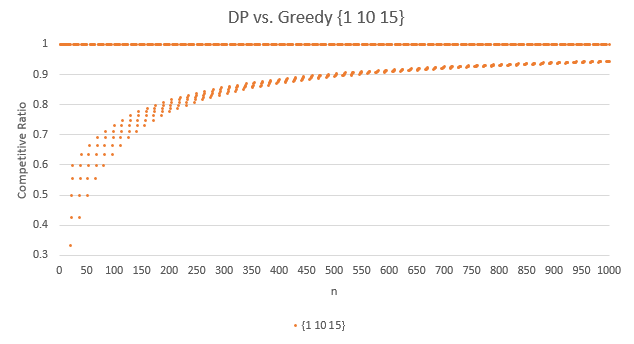
\includegraphics{11015} \\
					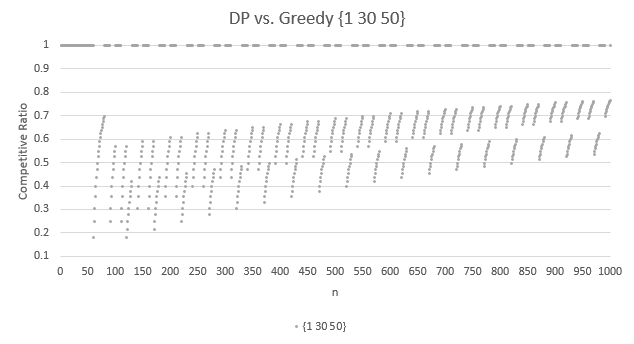
\includegraphics{13050} \\
					
			
			\end{enumerate}
%2d
		\item
			\begin{enumerate}[(i)]
	%2d.i
				\item
					\textbf{Optimal Greedy Proof for US Coin Denominations:} \textit{\{1, 5, 10, 25, 50\}} \\
						\hspace*{.5cm}
						For $ 1 \leq k \leq m $ prove that $ D_k + D_{k-1} - 1 $ yields the fewest coins for $ \{1...D_k\} and \{1..., D_{k-2}, D_{k-1}\} $. If $ \{1..., D_{k-2}, D_{k-1}\} $ yields fewer number of coins, then greedy fails. \\
						
						\hspace*{.5cm}
						Using \{1, 5, 10, 25, 50\}: \\
							\hspace*{.5cm}
							Highest value = 50 + 25 - 1 = 74 \textrightarrow 7 coins \\
							\hspace*{.5cm}
							Removing highest denomination: \{1, 5, 10, 25\} \\
							\hspace*{.5cm}
							74 \textrightarrow 8 coins \\
							\hspace*{.5cm}
							Highest value = 25 + 10 - 1 = 34 \textrightarrow 6 coins \\
							\hspace*{.5cm}
							Removing highest denomination: \{1, 5, 10\} \\
							\hspace*{.5cm}
							34 \textrightarrow 7 coins \\
							\hspace*{.5cm}
							Highest value = 10 + 5 - 1 = 14 \textrightarrow 5 coins \\
							\hspace*{.5cm}
							Remove highest denomination: \{1, 5\} \\
							\hspace*{.5cm}
							14 \textrightarrow 6 coins \\
							\hspace*{.5cm}
							Highest value = 5 + 1 - 1 = 5 \textrightarrow 1 \\
							\hspace*{.5cm}
							Remove highest denomination: \{1\} \\
							\hspace*{.5cm}
							5 \textrightarrow 6 coins \\
							
							$ \therefore $ Greedy minimizes number of coins for \{1, 5, 10, 25, 50\} since greedy picks the fewest number of coins for the denominations. \\
							
							
					
	%2d.ii
				\item
					\textbf{Greedy 2x, 10x vs. DP} \\
					\hspace*{.5cm}
						\begin{tabular}{ |c|c||c|c|c| }
							\hline
							\multicolumn{5}{|c|}{\textbf{Minimum Number Coins}} \\
							\hline
							Denomination & $ n $ & DP & Greedy & Greedy/DP \\
							\hline
							\{1, 10, 25\} & 30 & 3 & 6 & $ \frac{6}{3}=2 $ \\ 
							\hline
							\{1, 43, 100\} & 129 & 3 & 30 & $ \frac{30}{3}=10 $ \\ 
							\hline
						\end{tabular}
%1, 43, 100 | 129 : 30/3	
%1, 31, 64 | 93 : 30/3			
			
			\end{enumerate}
				
		\end{enumerate}


\end{enumerate}

\end{document}
